\documentclass{beamer}
\usepackage{relsize}
\usepackage{color}

\usepackage{listings}
\usetheme{CambridgeUS}
%\usepackage{beamerthemesplit} % new 
\usepackage{enumitem}
\usepackage{amsmath}                    % See geometry.pdf to learn the layout options. 
\usepackage{amsthm}                   % See geometry.pdf to learn the layout options. There 
\usepackage{amssymb}                    % See geometry.pdf to learn the layout options. 
\usepackage[utf8]{inputenc} 
\usepackage{graphicx}
\usepackage[english,bulgarian]{babel}

\lstset{language=C++,
                basicstyle=\ttfamily,
                keywordstyle=\color{blue}\ttfamily,
                stringstyle=\color{red}\ttfamily,
                commentstyle=\color{green}\ttfamily,
                morecomment=[l][\color{magenta}]{\#}
}

\newtheorem{mydef}{Дефиниция}[section]
\newtheorem{lem}{Лема}[section]
\newtheorem{thm}{Твърдение}[section]

\DeclareMathOperator{\restrict}{\upharpoonright}

\setitemize{label=\usebeamerfont*{itemize item}%
  \usebeamercolor[fg]{itemize item}
  \usebeamertemplate{itemize item}}

\setbeamercovered{transparent}



\begin{document}
\title[Увод в курса]{Въведение в курса. Програми, езици от високо ниво, базова структура на програма, променливи, вход и изход, условен оператор и цикъл, бройни системи, Машини на Тюринг} 
\author{Калин Георгиев} 
\frame{\titlepage} 

\section{Какво е програмиране} 
\subsection{Идея}

\frame{\frametitle{Програмиране?} 

\begin{figure}
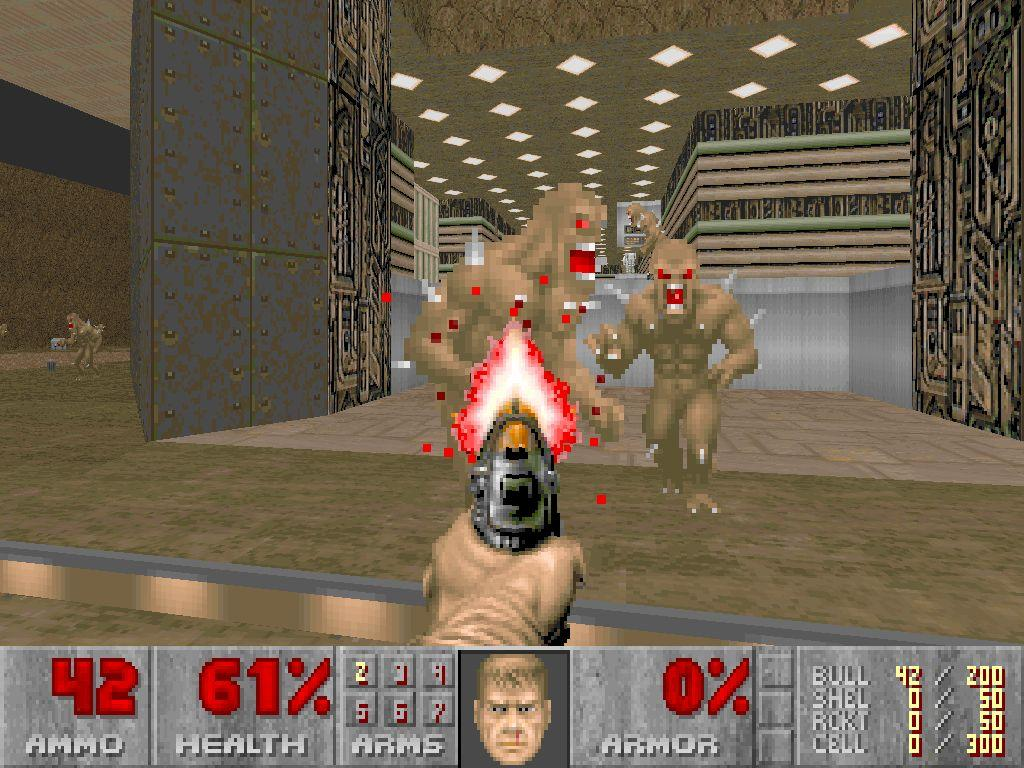
\includegraphics[width=9.5cm]{images/doom}
\end{figure}
  
}


\frame{\frametitle{Как работи?} 

\begin{figure}
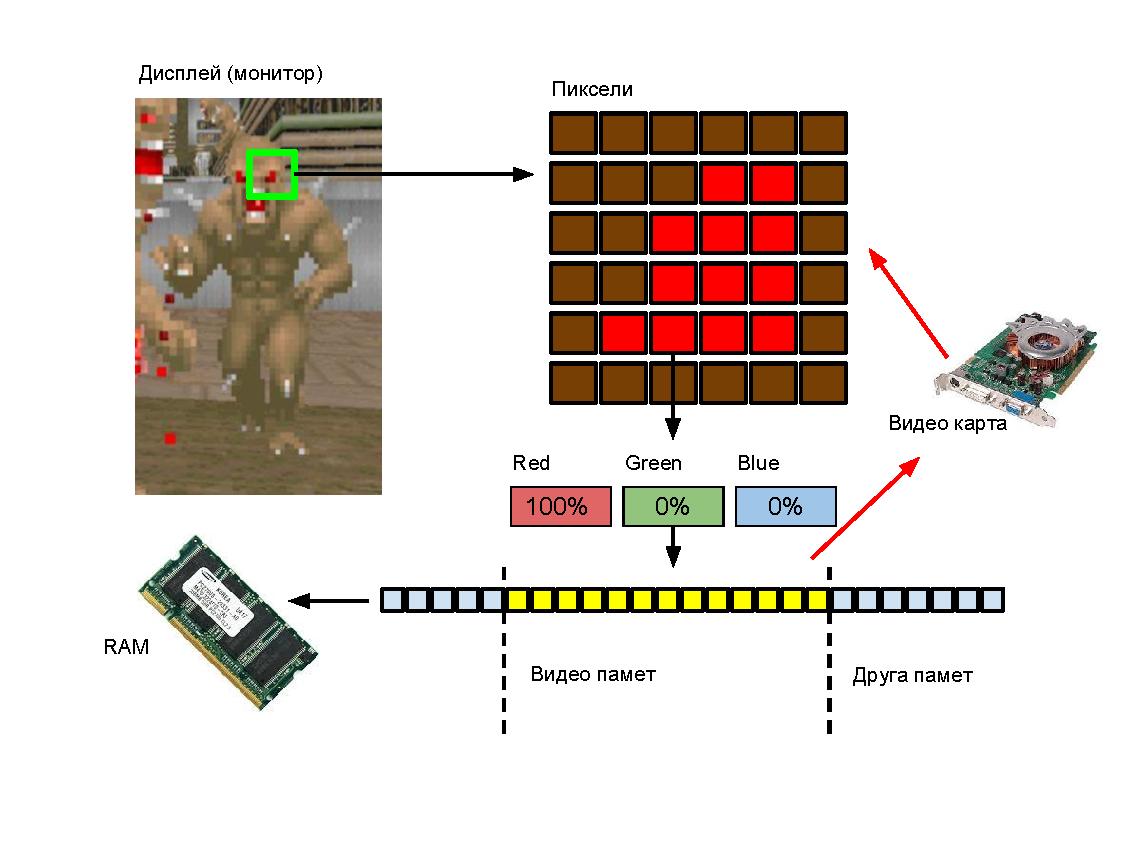
\includegraphics[width=9.5cm]{images/fig_display_memory}
\end{figure}
  }



\frame{\frametitle{Програми} 

\begin{figure}
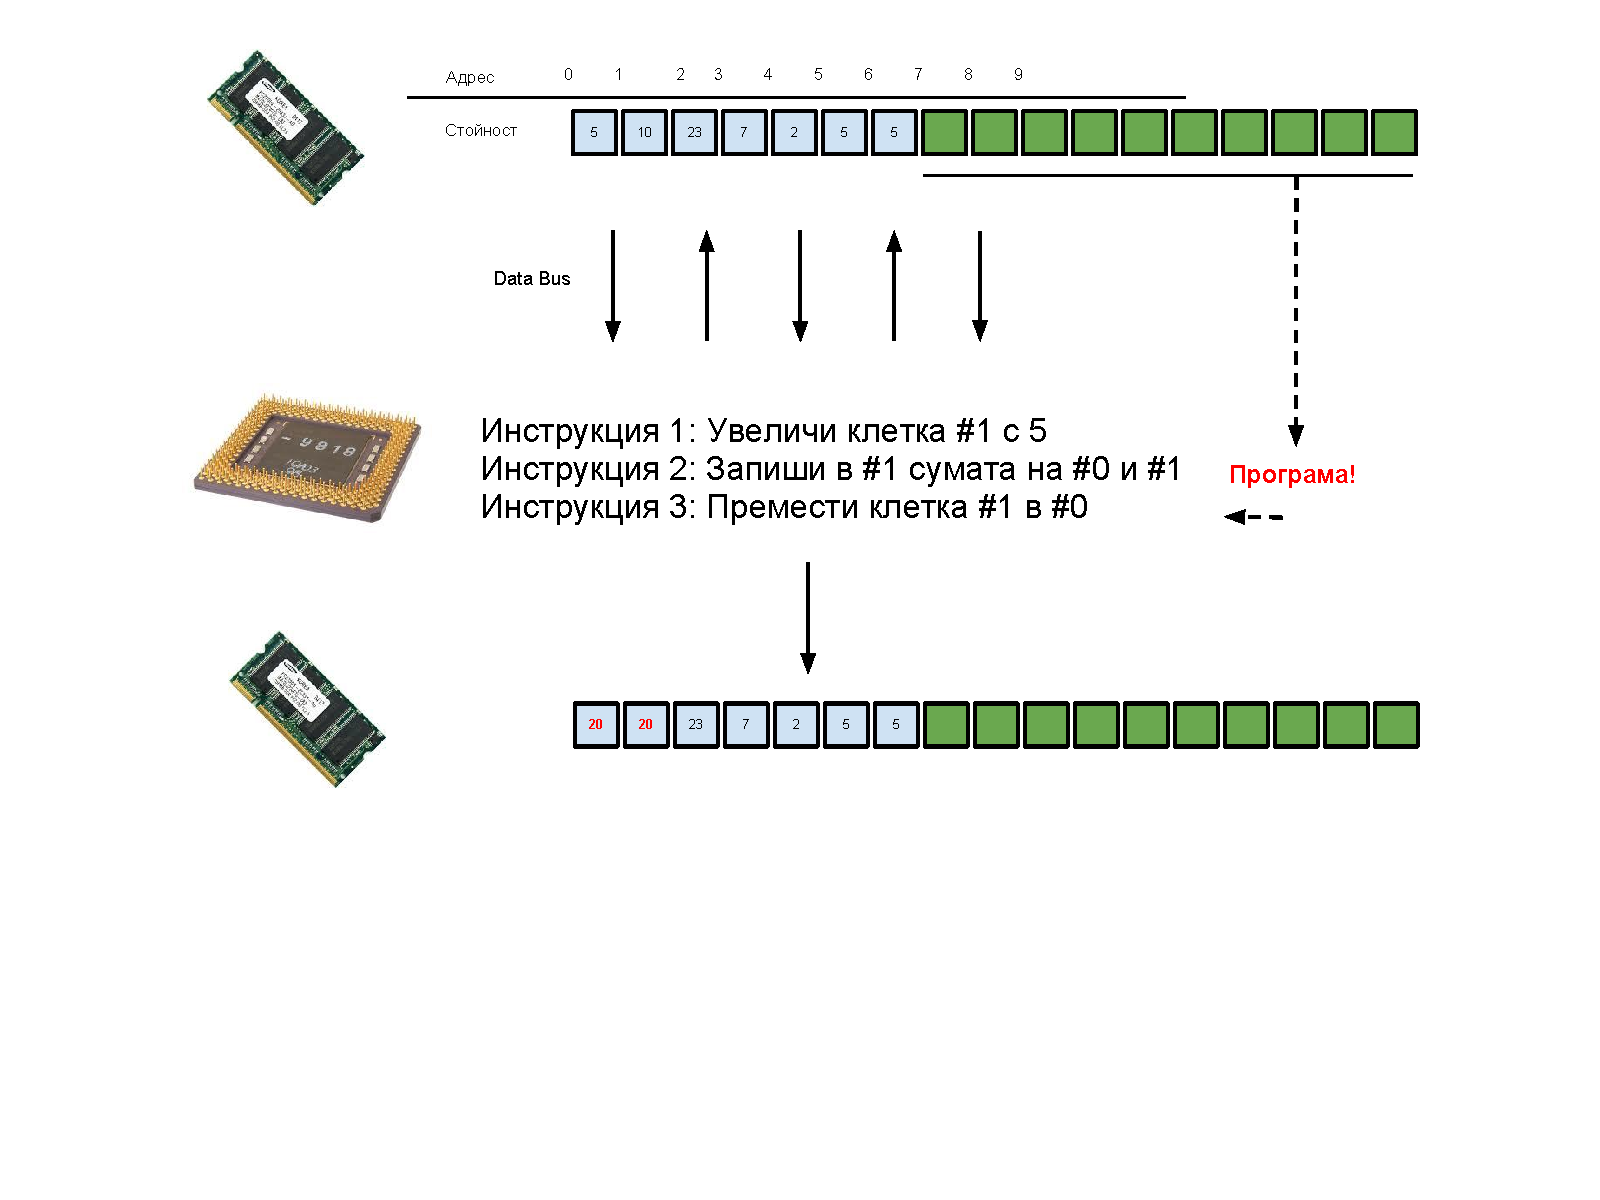
\includegraphics[width=12.5cm]{images/fig_program}
\end{figure}
}

\begin{frame}[fragile]
\frametitle{Език от високо ниво}

\begin{columns}
  \begin{column}{0.2\textwidth}
\begin{verbatim}

  int a = 5;
  int b = 10;

  b = b + 5;
  b = a + b;
  a = b;



  КОМПИЛАТОР--->

\end{verbatim}
  \end{column}
  \begin{column}{0.8\textwidth}
\begin{figure}
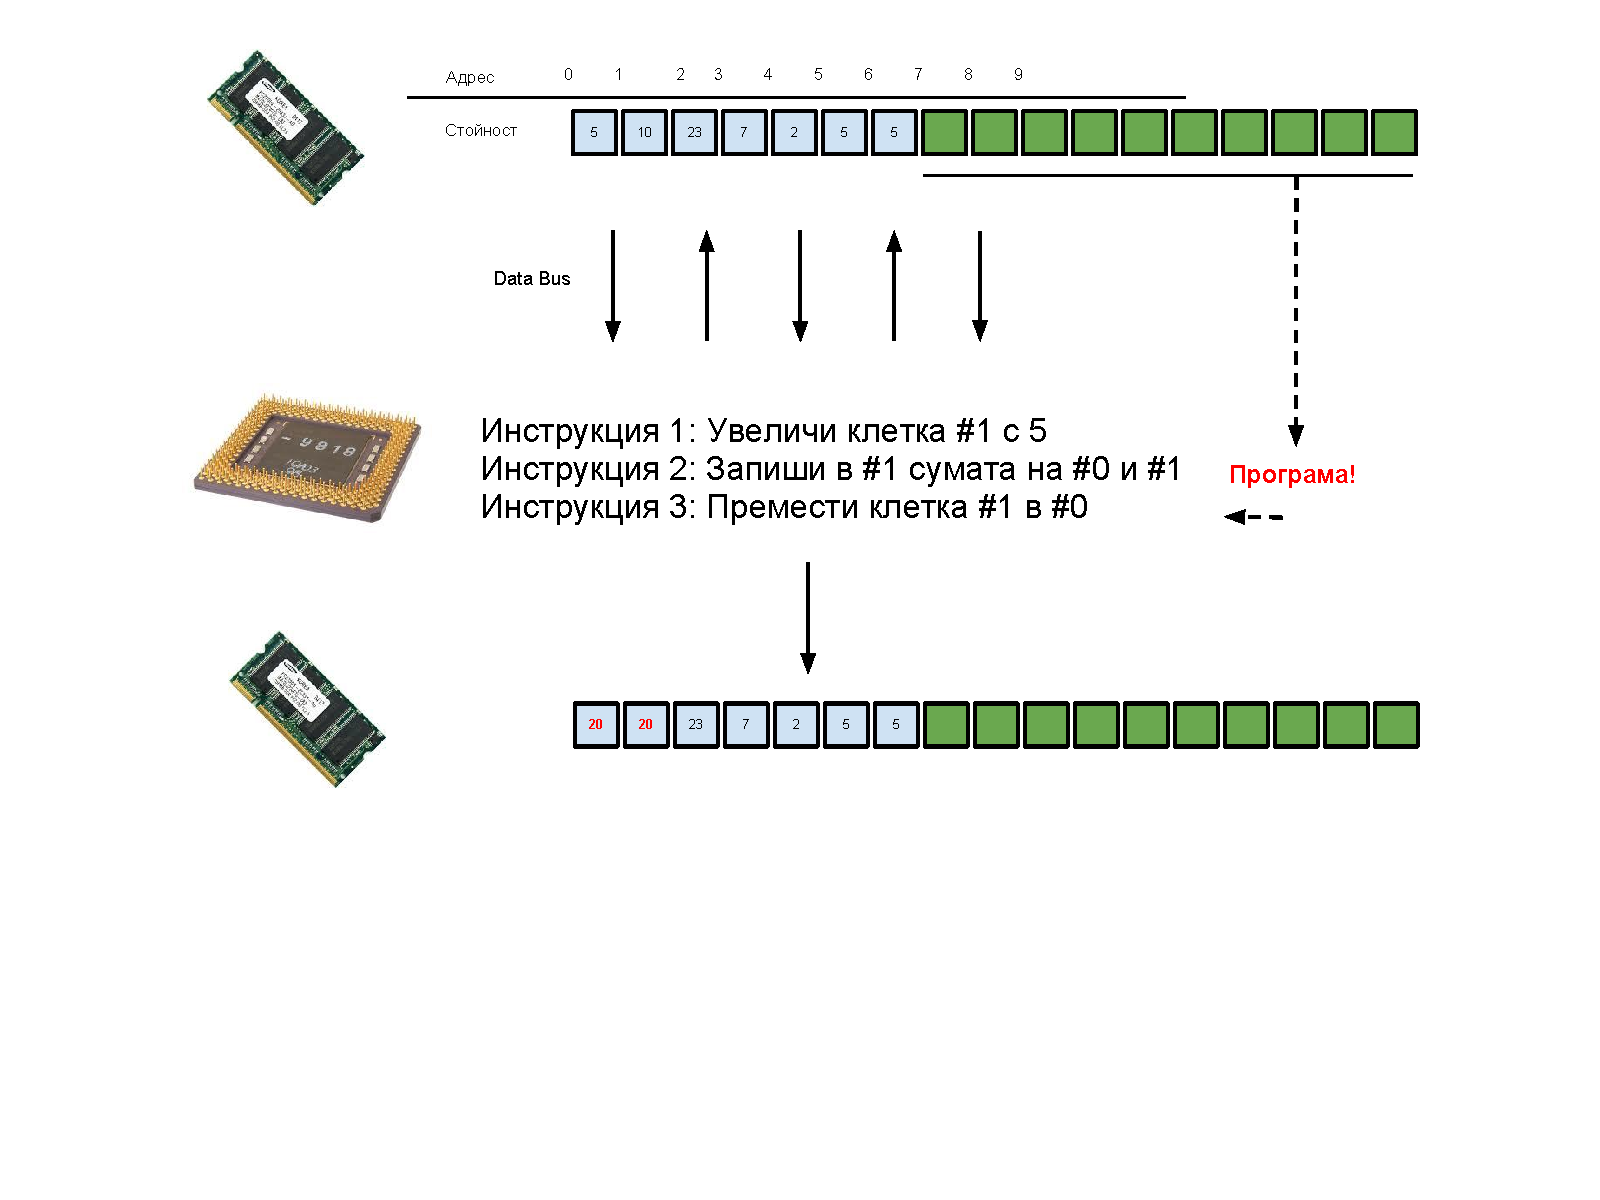
\includegraphics[width=10.5cm]{images/fig_program}
\end{figure}

  \end{column}
\end{columns}


\end{frame} 

\begin{frame}[fragile]
\frametitle{Променливи}


\begin{columns}[t]
  \begin{column}{0.7\textwidth}

\begin{itemize}
\item Стойност
\begin{lstlisting}
int a = 5;
int b = 10;
\end{lstlisting}
\item Адрес
\item Присвояване на стойност
\begin{lstlisting}
b = a + b;
\end{lstlisting}
\item Последователност на операциите
\begin{lstlisting}
int a = 5;
int b = 10;
b = a + b;
b = a + b;
\end{lstlisting}
\end{itemize}

  \end{column}



  \begin{column}{0.4\textwidth}
\begin{figure}
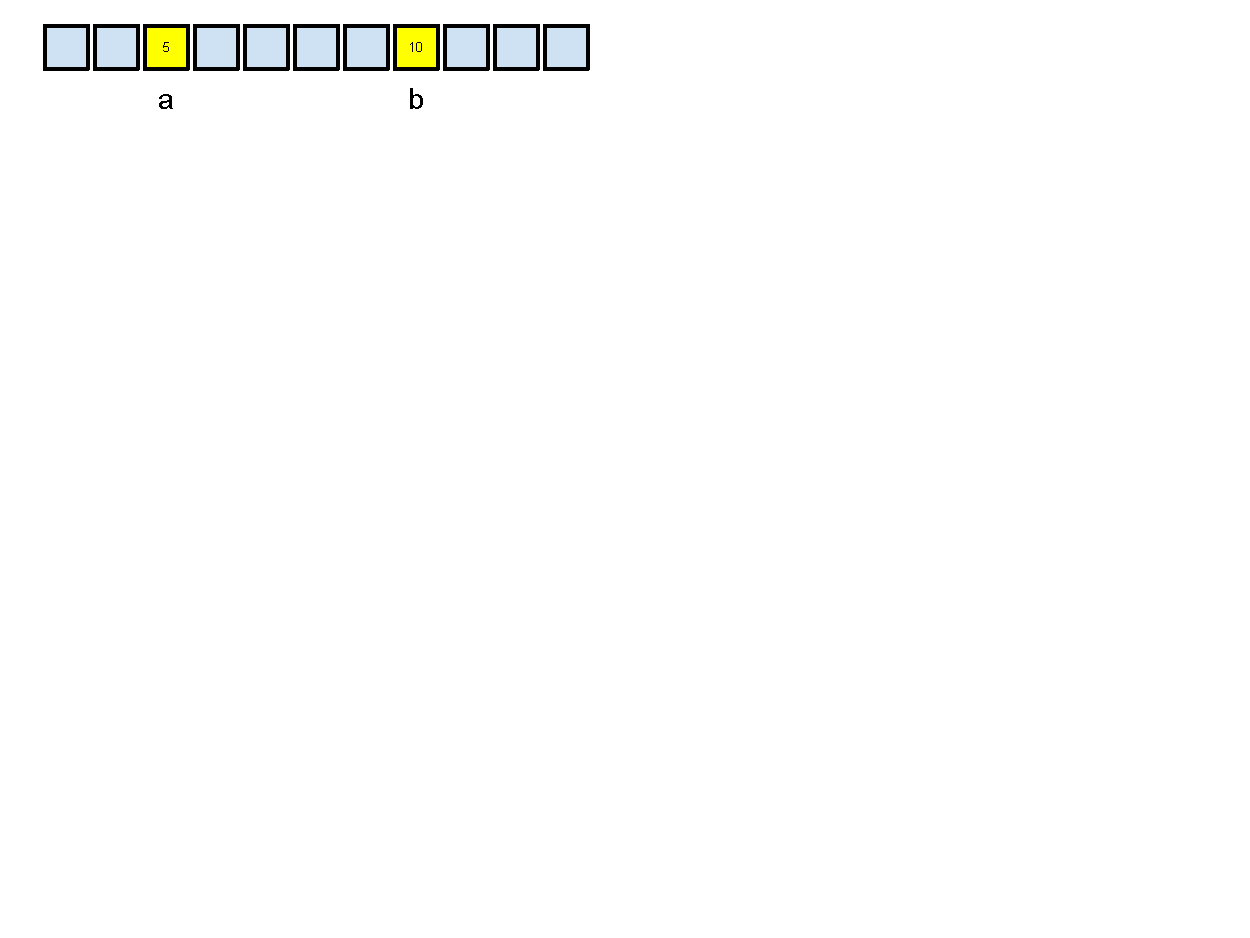
\includegraphics[width=8.5cm]{images/fig_variables}
\end{figure}
  \end{column}
\end{columns}

\end{frame}

\subsection{C++} 

\begin{frame}
\centerline{Език за програмиране C++}
\end{frame}


\begin{frame}[fragile]
\frametitle{Базова структура. Вход/изход}

\begin{columns}[t]
  \begin{column}{0.2\textwidth}
\relscale{0.63}
\begin{lstlisting}
#include <iostream>
using namespace std;

int main ()
{
  
  int a;

  cout << "Please, input the value of a=";
  cin >> a;
  cout << "a+5=" << a+5 << endl;

  return 0;

}
\end{lstlisting}
\relscale{1}

  \end{column}
  \begin{column}{0.8\textwidth}
\begin{figure}
\flushright
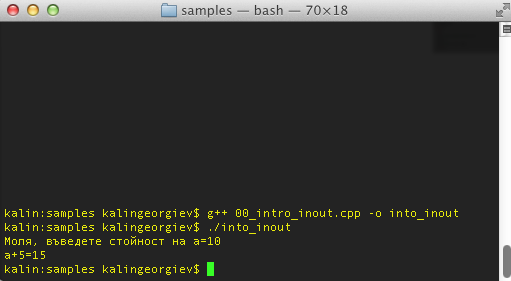
\includegraphics[width=6cm]{images/sample_inout}
\end{figure}
\begin{itemize}
\item Променлива
\item Константи: низови, числови
\item Аритметични операции
\item Конзола
\end{itemize}

  \end{column}
\end{columns}


\end{frame} 

\begin{frame}[fragile]
\frametitle{Пример: Средно аритметично}

\relscale{0.7}
\begin{lstlisting}
#include <iostream>
using namespace std;

int main ()
{
  
  int a,b,c;  //DOUBLE!!!

  cout << "Please, input the value of a=";
  cin >> a;
  cout << "Please, input the value of b=";
  cin >> b;
  cout << "Please, input the value of c=";
  cin >> c;
  
  cout << "average=" << (a+b+c)/3 << endl;

  return 0;

}
\end{lstlisting}

\end{frame} 


\begin{frame}[fragile]
\frametitle{Условен оператор}
\begin{itemize}
\item Проверка на условие: 
\relscale{0.7}
\begin{lstlisting}
int a;

cin >> a;

if (a > 5) {
   cout << "a is greater than 5";
} else {
   cout << "a is less than or equal to 5";
}
\end{lstlisting}
\relscale{1}
\item Прости видове условия за числа: >, >=, <, <=, ==, !=
\end{itemize}

\end{frame} 

\begin{frame}[fragile]
\frametitle{Вложени оператори}

\setbeamercovered{opaque}


\relscale{0.7}
\begin{columns}
  \begin{column}{0.5\textwidth}
  \begin{lstlisting}
int a = 701;

if (a > 20){
  if (a < 200){
    cout << "CASE 1";
  } else if (a < 700) {
    cout << "CASE 2";
  }} else {
    cout << "CASE 3";
  }


\end{lstlisting}
  \end{column}

\pause

  \begin{column}{0.5\textwidth}
  \begin{lstlisting}
int a = 701;

if (a > 20){
  if (a < 200){
    cout << "CASE 1";
  } 
  else 
     if (a < 700) {
       cout << "CASE 2";
     }
} 
else {
  cout << "CASE 3";
}
\end{lstlisting}
  \end{column}
\end{columns}

\setbeamercovered{transparent}


\end{frame}


\begin{frame}[fragile]
\frametitle{Пример: най-голямото от 3 числа}

\relscale{0.5}

\begin{columns}[t]
  \begin{column}{0.3\textwidth}
\begin{lstlisting}
if (a > b){
  if (b > c){
    cout << "max = " << a << endl;
  } else if (a > c)
    cout << "max = " << a << endl;    
  } else {
    cout << "max = " << c << endl;
  }
} else //b >= a { 
  if (a > c){
    cout << "max = " << b << endl;
  } else if (b > c)
    cout << "max = " << b << endl;    
  } else {
    cout << "max = " << c << endl;
  }
}

\end{lstlisting}

  \end{column}

\pause
  \begin{column}{0.3\textwidth}
\begin{lstlisting}
if (a > b){
  if (b > c || a > c){
      cout << "max = " << a << endl;  
  } else {   
      cout << "max = " << c << endl;  
  }
} else {
  if (a > c || b > c){
      cout << "max = " << b << endl;  
  } else {   
      cout << "max = " << c << endl;  
  }  
}
\end{lstlisting}

\pause

\begin{lstlisting}
if (a > b && a > c){
  cout << "max = " << a << endl; 
} else if (b > a && b > c) {
  cout << "max = " << b << endl; 
} else {
  cout << "max = " << c << endl; 
}
\end{lstlisting}
  \end{column}
\end{columns}


\end{frame}


\begin{frame}[fragile]
\frametitle{Булеви (логически) операции AND ($\wedge$) и OR ($\vee$)}

\begin{center}
  

\begin{tabular}{ c c }

\begin{tabular}{ c | c  c }
  \hline                        
  \&\&  & true  & false \\ \hline  
  true  & true  & false \\
  false & false & false \\
  
\end{tabular} &

\begin{tabular}{ c | c  c }
  \hline                        
  ||  & true  & false \\ \hline  
  true  & true  & true \\
  false & true & false \\
  
\end{tabular}

\end{tabular}
\end{center}



\end{frame}


\begin{frame}[fragile]
\frametitle{Пример: Корени на $ax^2+bx+c=0$}
\relscale{0.7}

\begin{lstlisting}
double a, b, c;

cin >> a >> b >> c;

int D = b*b - 4*a*c;

if (D < 0){
  cout << "NO roots!";
} else if (D == 0) {
  cout << "ONE root, x = " << (-b)/2*a << endl;
} else {
  cout << "TWO roots, x1 = " << (-b-sqrt(D))/2*a << endl <<
                     "x2 = " << (-b+sqrt(D))/2*a << endl;
}

\end{lstlisting}

\relscale{1}

\end{frame}


\subsection{For} 

\begin{frame}
\centerline{Циклични процеси}
\end{frame}



\begin{frame}[fragile]
\frametitle{Пример: Средно аритметично (отново)}

\relscale{0.7}
\begin{lstlisting}
#include <iostream>
using namespace std;

int main ()
{
  
  int a,b,c;  //DOUBLE!!!

  cout << "Please, input the value of a=";
  cin >> a;
  cout << "Please, input the value of b=";
  cin >> b;
  cout << "Please, input the value of c=";
  cin >> c;
  
  cout << "average=" << (a+b+c)/3 << endl;

  return 0;

}
\end{lstlisting}

\end{frame} 

\begin{frame}[fragile]
\frametitle{Пример: Средно аритметично на 10 числа}

\relscale{0.7}
\begin{lstlisting}
#include <iostream>
using namespace std;

int main ()
{
  
  int number, sum = 0;




  for (int counter = 0; counter < 10; counter++){

    cout << "Please enter number #" << counter << ":";
    cin >> number;
    sum = sum + number;

  }

  cout << "The average is " << sum / 10;

}
\end{lstlisting}

\end{frame} 

\begin{frame}[fragile]
\frametitle{Пример: Средно аритметично на N числа}

\relscale{0.7}
\begin{lstlisting}
#include <iostream>
using namespace std;

int main ()
{
  
  int number, sum = 0, numbersCount;

  cout << "Numbers count = ";
  cin >> numbersCount;

  for (int counter = 0; counter < numbersCount; counter++){

    cout << "Please enter number #" << counter << ":";
    cin >> number;
    sum = sum + number;

  }

  cout << "The average is " << sum / numbersCount;

}
\end{lstlisting}

\end{frame} 


\subsection{Теория} 

\begin{frame}
\centerline{Съвсем малко теория}
\end{frame}

\subsection{Бройни системи} 


\begin{frame}[fragile]
\frametitle{Бройни системи}

\textbf{Число (0x10)}

\begin{tabular}{ c | c | c  c}
   2 & 3 & 4 & = $2 * 10^2 + 3 * 10 + 4$ \\
\end{tabular} 

\pause

\begin{itemize}
  \item Какво става, ако имаме не 10, а 16 цифри 
\pause
  \item 0,1,2,3,4,5,6,7,8,9,... ???
 \pause
  \item A,B,C,D,E,F 

\end{itemize}

\pause

\textbf{Число (0x16)}

\begin{tabular}{ c | c | c  c}
   2 & 3 & 4 & = $2 * 16^2 + 3 * 16 + 4$ \\
\end{tabular} 

\begin{itemize}
  \item Ами ако имаме само две цифри? 
\end{itemize}


\pause

\textbf{Число (Binary)}

\begin{tabular}{ c | c | c  c}
   1 & 0 & 1 & = $1 * 2^2 + 0 * 2 + 1$ \\
\end{tabular} 

\pause

\begin{itemize}
  \item Защо бихме се ограничили до две цифри?
\end{itemize}




\end{frame}


\subsection{Модели} 


\begin{frame}[fragile]
\frametitle{Машини на Тюринг}


\begin{center}
  
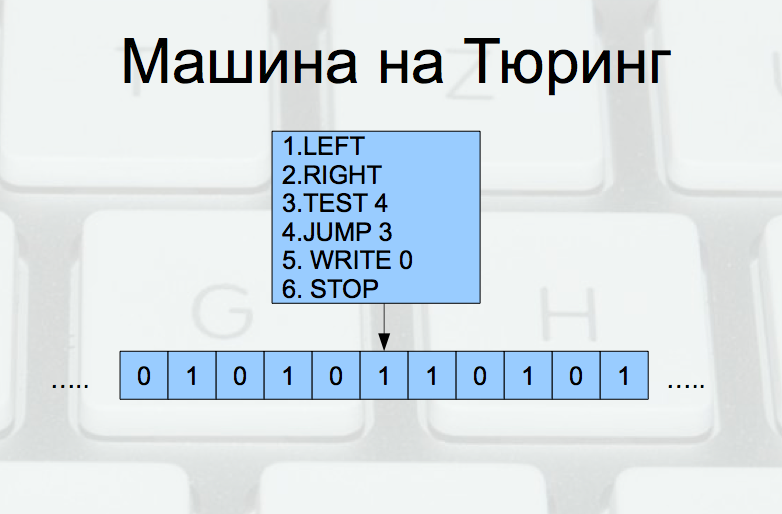
\includegraphics[width=9.5cm]{images/turing}

\end{center}

\end{frame}


\end{document}




\begin{columns}[t]
  \begin{column}{0.2\textwidth}

\relscale{0.63}
\begin{lstlisting}
\end{lstlisting}
\relscale{1}

  \end{column}
  \begin{column}{0.8\textwidth}

  \end{column}
\end{columns}

